
%(BEGIN_QUESTION)
% Copyright 2008, Tony R. Kuphaldt, released under the Creative Commons Attribution License (v 1.0)
% This means you may do almost anything with this work of mine, so long as you give me proper credit

A technician is troubleshooting a power supply circuit with no DC output voltage.  The output voltage is supposed to be 15 volts DC, but instead it is actually outputting nothing at all (zero volts):

$$\includegraphics[width=15.5cm]{i03176x01.eps}$$

The technician measures 120 volts AC between test points TP1 and TP3.  Based on this voltage measurement and the knowledge that there is zero DC output voltage, identify two possible faults (either one of which could account for the problem and all measured values in this circuit), and also identify two circuit elements that could not possibly be to blame (i.e. two things that you know {\it must} be functioning properly, no matter what else may be faulted).  The circuit elements you identify as either possibly faulted or properly functioning can be wires, traces, and connections as well as components.  Be as specific as you can in your answers, identifying both the circuit element and the type of fault.

\begin{itemize}
\goodbreak
\item{} Circuit elements that are possibly faulted
\item{1.} 
\item{2.} 
\end{itemize}

\begin{itemize}
\goodbreak
\item{} Circuit elements that must be functioning properly
\item{1.} 
\item{2.} 
\end{itemize}

\vfil 

\underbar{file i03176}
\eject
%(END_QUESTION)





%(BEGIN_ANSWER)

This is a graded question -- no answers or hints given!

%(END_ANSWER)





%(BEGIN_NOTES)

The good 120 VAC measurement between TP1 and TP3 tells us AC power is making it all the way to the primary side of the transformer, therefore the fuse must be good and the power source okay, as well as all traces between the cord and those test points.

\vskip 10pt

\begin{itemize}
\goodbreak
\item{} Circuit elements that are possibly faulted
\item{1.} Transformer primary winding (open)
\item{2.} Transformer secondary winding (open)
\item{3.} Diodes (multiple would have to fail open)
\item{4.} Poor solder joint anywhere in the current-carrying path of the low-voltage side of the circuit
\item{5.} Open PCB trace anywhere in the current-carrying path of the low-voltage side side of the circuit
\end{itemize}

\begin{itemize}
\goodbreak
\item{} Circuit elements that must be functioning properly
\item{1.} AC power source (wall receptacle)
\item{2.} Fuse
\item{3.} PCB trace from TP1 to power cord
\item{4.} PCB trace from fuse holder to power cord (TP2)
\item{5.} PCB trace from TP3 to fuse holder
\end{itemize}


%INDEX% Troubleshooting review: electric circuits

%(END_NOTES)


